% =================================================================================================
% File:			desc_dp.tex
% Description:	Definisce la sezione relativa all'appendice sui design pattern
% Created:		2015-03-27
% Author:		Tesser Paolo
% Email:		tesser.paolo@mashup-unipd.it
% =================================================================================================
% Modification History:
% Version		Modifier Date		Change											Author
% 0.0.1 		2015-03-27 			creato scheletro								Tesser Paolo
% =================================================================================================
% 0.0.2			2015-04-10			aggiunto scheltro per altri DP trovati			Tesser Paolo
% =================================================================================================
%

% CONTENUTO DEL CAPITOLO



\section{Descrizione Design Pattern} % (fold)
\label{sec:descdp}
	\subsection{Design pattern architetturali} % (fold)

		\subsubsection{Three-Tier} % (fold)
		TO DO (grafico)
		\begin{itemize}
			\item \textbf{Scopo}: TO DO;
			\item \textbf{Motivazione}: TO DO;
			\item \textbf{Applicabilità}: TO DO;
		\end{itemize}
		% subsubsection three_tier (end)

		\subsubsection{MVC} % (fold)
		\begin{figure}[htbp]
			\centering
			\centerline{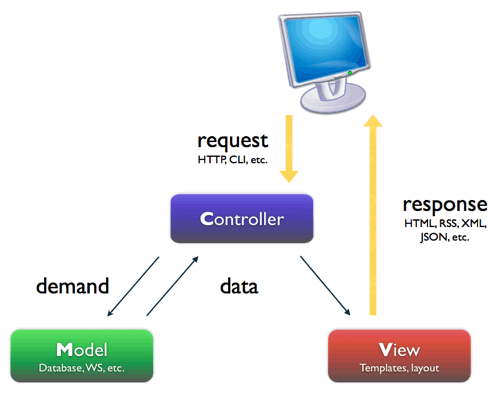
\includegraphics[scale=0.6]{./images/mvc.png}}
			\caption{Design pattern architetturale - MVC}
		\end{figure}
		TO DO (da rifare grafico tramite Astah in maniera che sia conforme agli altri grafici, può essere sempre generale a livello di nomi, ma così viene più elegante)

		\begin{itemize}
			\item \textbf{Scopo}: TO DO;
			\item \textbf{Motivazione}: TO DO;
			\item \textbf{Applicabilità}: TO DO;
		\end{itemize}

		TO DO (da rifare inquadrandolo sullo scheletro sovrastante) \newline

		Il pattern è basato sulla separazione dei compiti fra i componenti software che interpretano tre ruoli principali:
		\begin{itemize}
			\item \textbf{Model} che fornisce i metodi per accedere ai dati utili all'applicazione;
			\item \textbf{View} che visualizza i dati contenuti nel model e si occupa dell'interazione con utenti e agenti;
			\item \textbf{Controller} che riceve i comandi dell'utente (in genere attraverso il view) e li attua modificando lo stato degli altri due componenti.
		\end{itemize}
		\noindent
		Questo schema implica anche la tradizionale separazione fra la logica applicativa (in questo contesto spesso chiamata ``logica di business''), a carico del controller e del model, e l'interfaccia utente a carico del view. I dettagli delle interazioni fra questi tre oggetti software dipendono molto dalle tecnologie usate (linguaggio di programmazione, eventuali librerie, middleware e via dicendo) e dal tipo di applicazione (per esempio se si tratta di un'applicazione web, o di un'applicazione desktop). Quasi sempre la relazione fra view e model è descrivibile anche come istanza del pattern Observer. A volte, quando è necessario cambiare il comportamento standard dell'applicazione a seconda delle circostanze, il controller implementa anche il pattern Strategy.

		% subsubsection mvc (end)

		\subsubsection{MVVM} % (fold)
		TO DO (grafico)
		\begin{itemize}
			\item \textbf{Scopo}: TO DO;
			\item \textbf{Motivazione}: TO DO;
			\item \textbf{Applicabilità}: TO DO;
		\end{itemize}
		% subsubsection mvvm (end)

		\subsubsection{Dependency Injection} % (fold)
		TO DO (grafico)
		\begin{itemize}
			\item \textbf{Scopo}: TO DO;
			\item \textbf{Motivazione}: TO DO;
			\item \textbf{Applicabilità}: TO DO;
		\end{itemize}
		% subsubsection dependency_injection (end)

	% subsection design_pattern_architetturali (end)


	\clearpage \newpage

	\subsection{Design pattern creazionali} % (fold)
		\subsubsection{Prototype Pattern} % (fold)

		TO DO (grafico)
		\begin{itemize}
			\item \textbf{Scopo}: TO DO;
			\item \textbf{Motivazione}: TO DO;
			\item \textbf{Applicabilità}: TO DO;
		\end{itemize}
		% subsubsection prototype_pattern (end)

		\subsubsection{Module Pattern} % (fold)
		TO DO (grafico)
		\begin{itemize}
			\item \textbf{Scopo}: TO DO;
			\item \textbf{Motivazione}: TO DO;
			\item \textbf{Applicabilità}: TO DO;
		\end{itemize}

		\subsubsection{Singleton} % (fold)
		TO DO (grafico)
		\begin{itemize}
			\item \textbf{Scopo}: TO DO;
			\item \textbf{Motivazione}: TO DO;
			\item \textbf{Applicabilità}: TO DO;
		\end{itemize}
		
		% subsubsection singleton (end)
		% subsubsection module_pattern (end)

	% subsection design_pattern_creazionali (end)

	\clearpage \newpage

	\subsection{Design pattern strutturali} % (fold)
		\subsubsection{Fa\c{c}ade} % (fold)
		TO DO (grafico)
		\begin{itemize}
			\item \textbf{Scopo}: TO DO;
			\item \textbf{Motivazione}: TO DO;
			\item \textbf{Applicabilità}: TO DO;
		\end{itemize}



	% subsection design_pattern_strutturali (end)

	\clearpage \newpage

	\subsection{Design pattern comportamentali} % (fold)
		\subsubsection{Page Controller} % (fold)
		TO DO (grafico)
		\begin{itemize}
			\item \textbf{Scopo}: TO DO;
			\item \textbf{Motivazione}: TO DO;
			\item \textbf{Applicabilità}: TO DO;
		\end{itemize}
		% subsubsection page_controller (end)

		\subsubsection{Template View} % (fold)
		TO DO (grafico)
		\begin{itemize}
			\item \textbf{Scopo}: TO DO;
			\item \textbf{Motivazione}: TO DO;
			\item \textbf{Applicabilità}: TO DO;
		\end{itemize}
		% subsubsection template_view (end)

	% subsection design_pattern_comportamentali (end)


% section descdp (end)